\documentclass[12pt,a4paper]{report}
\usepackage[utf8]{inputenc}
\usepackage[brazilian]{babel}
\usepackage[skip=1.2\baselineskip]{parskip}
\usepackage{amsfonts}
\usepackage{amsmath}
\usepackage{amssymb}
\usepackage{enumitem}
\usepackage{fancyhdr}
\usepackage{float}
\usepackage{geometry}
\usepackage{graphicx}
\usepackage{hyperref}
\usepackage{setspace}
\usepackage{tabularx}
\usepackage{titlesec}
\usepackage{tcolorbox}
\usepackage{tikz}
\usepackage[table]{xcolor}

\addto\captionsbrazilian{\renewcommand{\chaptername}{Seção}}

\pagestyle{fancy}
\fancyhf{} 
\fancyhead[C]{\leftmark} 
\fancyfoot[C]{\thepage} 

\hypersetup{
	colorlinks=true,
	linkcolor=blue,
	filecolor=magenta,      
	urlcolor=blue,
	pdftitle={Manual do Aplicativo LogoAX},
}

\geometry{top=2cm, bottom=2cm, left=2.5cm, right=2.5cm}

\begin{document}
	
	\begin{titlepage}
		\centering
		
		\pagenumbering{gobble}
			
		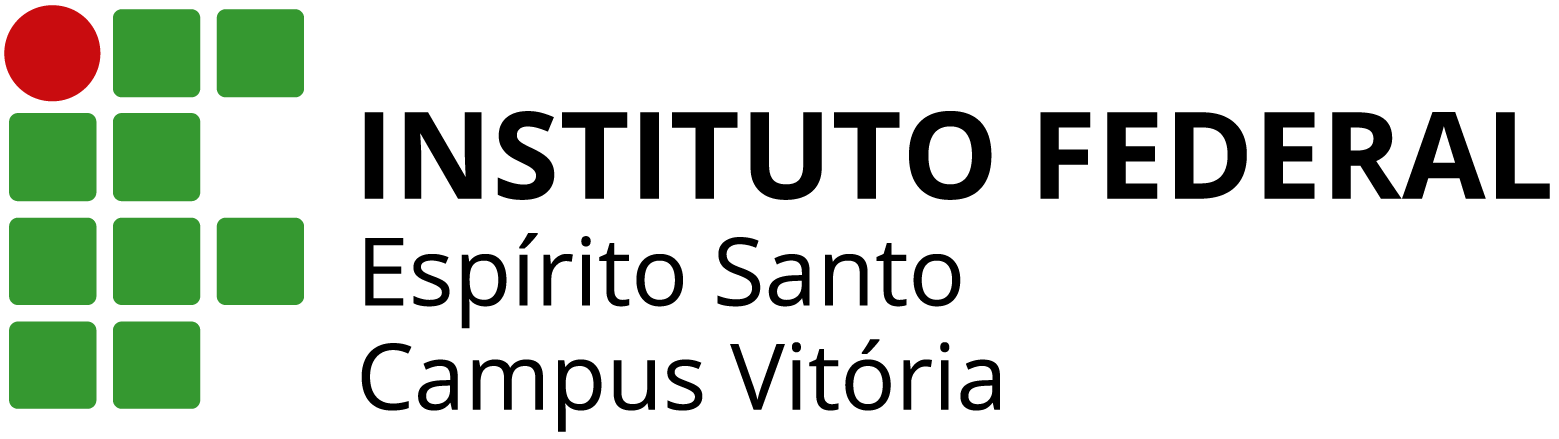
\includegraphics[width=8cm]{ifes.png}\\[1cm]
		
		{\Large \textbf{Instituto Federal do Espírito Santo}}\\[0.5cm]
		{\large \textbf{Tecnologias Digitais em Educação Matemática}}\\[0.5cm]
		
		\vspace{\fill}
		
		{\Huge \textbf{Manual do Aplicativo \textsc{LogoAX}}}\\[0.5cm]
		
		\vspace{\fill}
		
		{\Large Professor Alex Jordane}
		
		\vspace{\fill}
		
		{\large Vitória -- ES}\\[0.2cm]
		{\large 2026}
		
	\end{titlepage}
	
	\pagenumbering{arabic}
	
	\chapter*{Apresentação}
	\thispagestyle{empty}
		
	\setcounter{page}{1}
	
	Este manual foi estruturado para orientar o uso do \textsc{LogoAX} na disciplina Tecnologias Digitais em Educação Matemática. O objetivo deste material é fornecer uma referência direta para a compreensão dos comandos e da interface do aplicativo, servindo de apoio para as atividades da primeira fase das Tecnologias Digitais na Educação Matemática.
	
	O texto está organizado em duas seções: a descrição detalhada dos componentes visuais da tela e o mapeamento dos comandos operacionais da tartaruga, incluindo suas estruturas de repetição e blocos de procedimentos. 
	
	Cada seção apresenta as instruções de forma linear, indicando a sintaxe correta e os parâmetros necessários para a execução dos desenhos no palco virtual. Recomenda-se a consulta contínua a este guia durante o planejamento e a escrita dos roteiros no editor.
	
	A linguagem Logo foi desenvolvida no final da década de 1960 por Seymour Papert e sua equipe de pesquisadores. A pesquisa de Papert estabeleceu o uso da programação de computadores como um recurso para a aprendizagem e o desenvolvimento cognitivo.
	
	O \textsc{LogoAX} foi criado por Alex Jordane em colaboração com a inteligência artificial Gemini (versão 3.1 Pro). O sistema foi estruturado utilizando as linguagens \texttt{HTML} e \texttt{Python}, com a integração do interpretador \texttt{Skulpt} (\href{https://skulpt.org/}{https://skulpt.org/}).
	
	O aplicativo possui propósito educacional e seu acesso é exclusivo para estudantes da disciplina \textbf{Tecnologias Digitais em Educação Matemática}.
	
	\vspace{\fill}
	
	{\footnotesize
	\texttt{Este material foi elaborado em colaboração com a inteligência artificial Gemini, versão 3.1 Pro.} \\		
	\texttt{O compartilhamento e a reprodução deste material são permitidos, desde que a fonte e a autoria sejam citadas.}  \\		
	\texttt{Esta obra está licenciada com uma Licença Atribuição-NãoComercial-SemDerivações 4.0 Brasil.}
	\begin{center}
		
\includegraphics[width=4cm]{CC.png}
	\end{center}}
	
	
	\tableofcontents
	\thispagestyle{empty}

	\chapter{Interface Visual e Controles}
	
	A tela do \textsc{LogoAX} (Figura \ref{fig:tela}) está organizada para facilitar a exploração geométrica e a programação. O espaço é dividido em áreas com funções específicas, que trabalham de maneira integrada para dar movimento à tartaruga.
	
	% [INSERIR IMAGEM AQUI: Visão geral da tela do aplicativo]
	\begin{figure}[H]
	   \centering
		\caption{Visão geral do aplicativo Logo.}
		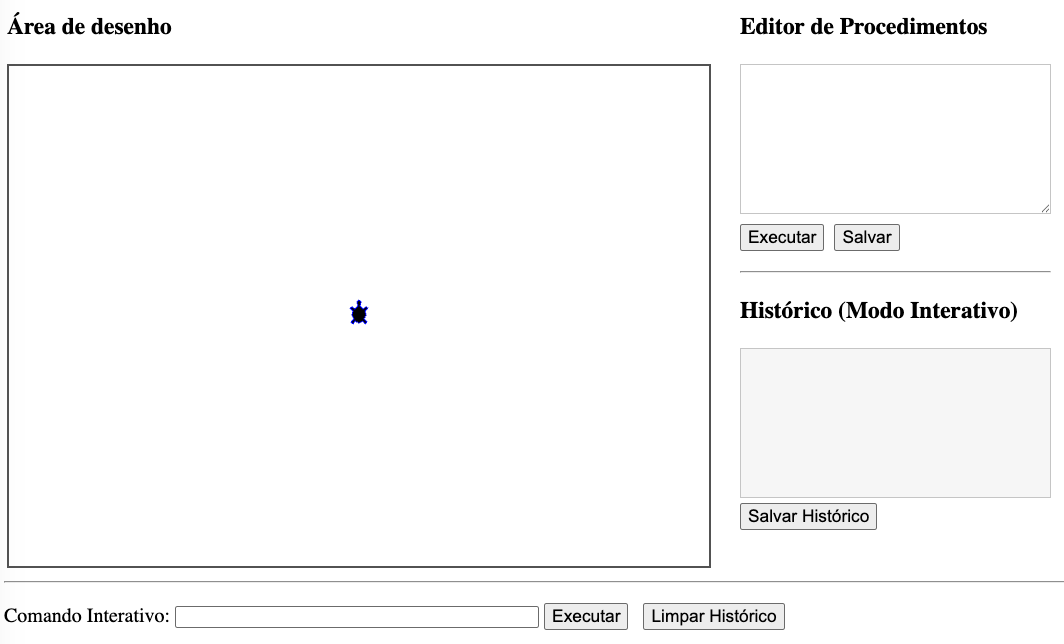
\includegraphics[width=0.8\textwidth]{imagem_tela_geral.png}
	    \label{fig:tela}
	\end{figure}
	
	\section{Área de Desenho}
	
	A Área de Desenho (Figura \ref{fig:area}) é o palco principal. É neste espaço que a tartaruga realiza seus movimentos, desenhando linhas e figuras geométricas conforme as instruções recebidas. A área possui limites fixos, garantindo uma proporção constante para a visualização dos traçados. O centro da tela representa a origem do plano, de onde a tartaruga inicia sua jornada.
	
	% [INSERIR IMAGEM AQUI: Destaque apenas da Área de Desenho com a tartaruga no centro]
	\begin{figure}[H]
		\centering
		\caption{Área de Desenho.}
		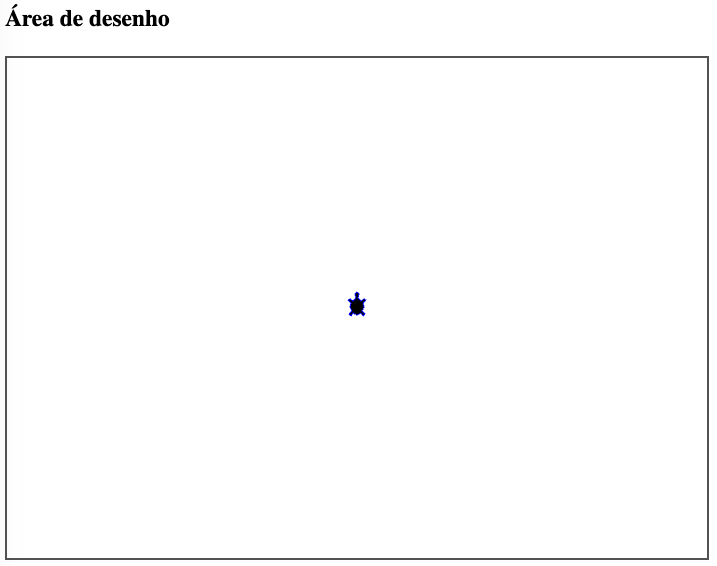
\includegraphics[width=0.6\textwidth]{imagem_area_desenho.png}
		\label{fig:area}
	\end{figure}
	
	\section{Editor de Procedimentos}
	
	O Editor de Procedimentos (Figura \ref{fig:editor}) é um espaço reservado para a escrita de roteiros mais longos e estruturados. Nele, é possível planejar um desenho completo e ensinar novos comandos para a tartaruga por meio da criação de procedimentos.
	
	Logo abaixo da caixa de texto, existem dois botões:
	\begin{itemize}
		\item \textbf{Executar:} Lê todo o texto escrito no editor, ensina os novos procedimentos à tartaruga e realiza a animação na Área de Desenho.
		\item \textbf{Salvar:} Permite que o código digitado seja baixado para o computador em um arquivo de texto, preservando a construção para uso futuro.
	\end{itemize}
	
	% [INSERIR IMAGEM AQUI: Destaque do Editor de Procedimentos e seus botões]
	\begin{figure}[H]
	    \centering
	    \caption{Editor de Procedimentos e seus respectivos botões.}
	    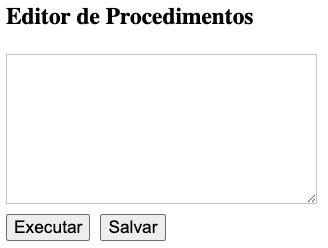
\includegraphics[width=0.5\textwidth]{imagem_editor.png}
	    \label{fig:editor}
	\end{figure}
	
	\section{Histórico (Modo Interativo)}
	
	O Histórico (Figura \ref{fig:historico}) funciona como a memória dos passos recentes. Toda vez que um comando é enviado para a tartaruga, ele é registrado nesta caixa, formando uma lista sequencial das ações realizadas no momento.
	
	Abaixo do painel, o botão \textbf{Salvar Histórico} possibilita o download dessa lista de passos em formato de texto, o que é oportuno para registrar testes e investigações.
	
	% [INSERIR IMAGEM AQUI: Destaque da caixa de Histórico]
	\begin{figure}[H]
	    \centering
	    \caption{Painel de Histórico.}
	    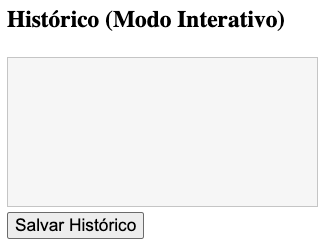
\includegraphics[width=0.5\textwidth]{imagem_historico.png}
	    \label{fig:historico}
	\end{figure}
	
	\section{Comando Interativo}
	
	A caixa de Comando Interativo (Figura \ref{fig:comandos}) estabelece o diálogo direto e imediato com a tartaruga. É o local para enviar instruções rápidas, passo a passo, acompanhando o resultado na tela instantaneamente.
	
	Para que a tartaruga obedeça à instrução digitada, é possível utilizar o botão \textbf{Executar} ou simplesmente pressionar a tecla \textbf{Enter} no teclado. 
	
	Ao lado, o botão \textbf{Limpar Histórico} esvazia a memória recente de comandos interativos e devolve a tartaruga para o centro da tela, apagando os traços feitos e deixando o palco pronto para uma nova exploração.
	
	% [INSERIR IMAGEM AQUI: Destaque da barra de Comando Interativo na parte inferior]
	\begin{figure}[H]
	    \centering
	    \caption{Barra de Comando Interativo e botões de controle.}
	    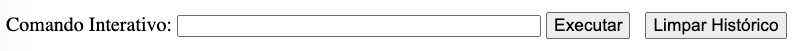
\includegraphics[width=0.7\textwidth]{imagem_comando_interativo.png}
	    \label{fig:comandos}
	\end{figure}
	
	\chapter{Comandos do Logo}
	
	\section{Comandos Básicos}
	
	Os comandos básicos controlam o movimento relativo e a rotação da tartaruga. O valor informado logo após o comando representa a quantidade de passos ou o ângulo em graus.
	
	\begin{itemize}
		\item \textbf{\texttt{pf \textit{n}}}: Move a tartaruga para frente \textit{n} passos.
		\item \textbf{\texttt{pt \textit{n}}}: Move a tartaruga para trás \textit{n} passos.
		\item \textbf{\texttt{pd \textit{a}}}: Gira a tartaruga para a direita em \textit{a} graus.
		\item \textbf{\texttt{pe \textit{a}}}: Gira a tartaruga para a esquerda em \textit{a} graus.
	\end{itemize}
	
	\section{Comandos de Tela}
	
	Estes comandos atuam na limpeza da área de desenho e no gerenciamento geral do ambiente.
	
	\begin{itemize}
		\item \textbf{\texttt{tat}} (tartaruga apaga tela): Apaga os desenhos, levanta a caneta, posiciona a tartaruga no centro do palco e a aponta para cima.
		\item \textbf{\texttt{lt}} (limpa tela): Recarrega a página do aplicativo, esvaziando a memória, o histórico e a Área de Desenho.
	\end{itemize}
	
	\section{Movimentação e Coordenadas}
	
	A Área de Desenho funciona como um plano cartesiano com dimensões de 700 pixels de largura por 500 pixels de altura (Figura \ref{fig:plano}). A origem desse plano, correspondente à coordenada $(0, 0)$, está localizada no centro da tela.
	
	A partir do centro, os limites espaciais da Área de Desenho são definidos da seguinte maneira:
	\begin{itemize}
		\item \textbf{Eixo X (horizontal):} Estende-se de $-350$ (borda esquerda) a $350$ (borda direita).
		\item \textbf{Eixo Y (vertical):} Estende-se de $-250$ (borda inferior) a $250$ (borda superior).
	\end{itemize}
	
	% [INSERIR IMAGEM AQUI: Esquema do plano cartesiano sobrepondo a Área de Desenho, destacando o centro (0,0) e os limites dos eixos]
	\begin{figure}[H]
	    \centering
	    \caption{Limites e coordenadas da Área de Desenho.}
	    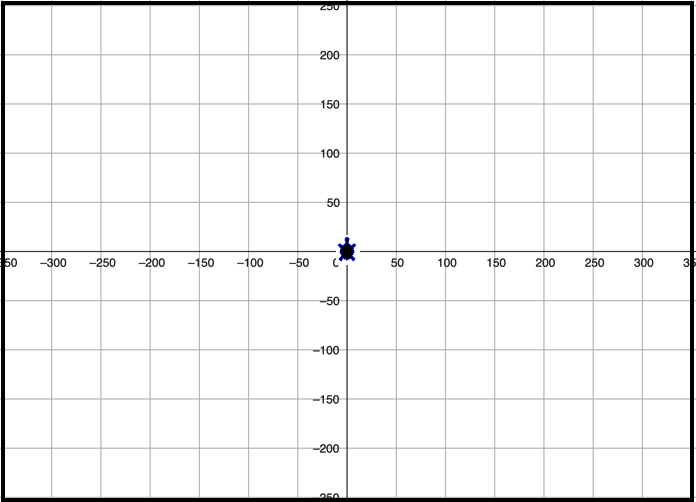
\includegraphics[width=0.7\textwidth]{imagem_plano_cartesiano.png}
	    \label{fig:plano}
	\end{figure}
	
	Os comandos a seguir utilizam essas coordenadas cartesianas e direções absolutas para orientar a tartaruga:
	
	\begin{itemize}
		\item \texttt{\textbf{mudepos \textit{x y}}}: Move a tartaruga diretamente para o ponto definido pelas coordenadas \textit{x} e \textit{y}.
		\item \textbf{\texttt{mudex \textit{x}}}: Altera apenas a posição horizontal da tartaruga para a coordenada \textit{x}.
		\item \texttt{\textbf{mudey \textit{y}}}: Altera apenas a posição vertical da tartaruga para a coordenada \textit{y}.
		\item \texttt{\textbf{centro}}: Move a tartaruga para a coordenada $(0, 0)$ e a aponta para a direção superior da tela.
		\item \texttt{\textbf{cima}}: Altera a direção da tartaruga, fazendo-a apontar estritamente para a parte superior da tela (ângulo de 90 graus), sem movê-la do lugar.
	\end{itemize}
	
	\section{Comandos do Lápis e Cores}
	
	Os comandos de lápis gerenciam o rastro deixado pela tartaruga durante seus deslocamentos e a cor da tinta.
	
	\begin{itemize}
		\item \textbf{\texttt{ul}} (use lápis): Encosta o lápis na tela. A tartaruga desenha ao se mover, usando a cor previamente definida.
		\item \textbf{\texttt{ub}} (use borracha): Configura o lápis para a cor branca de fundo e abaixa a caneta. A tartaruga apaga os traços por onde passa. \textbf{Esse comando não tem um bom resultado, evite usá-lo!}
		\item \textbf{\texttt{un}} (use nada): Levanta o lápis. A tartaruga se move sem deixar rastro.
		\item \textbf{\texttt{mudecl \textit{cor}}}: Altera a cor do traçado. O sistema aceita o nome da cor, seu número correspondente ou uma lista de valores RGB no formato \texttt{[R G B]}. Exemplo: \texttt{mudecl azul}, \texttt{mudecl 4} ou \texttt{mudecl [0 0 255]}.
	\end{itemize}
	
	A Tabela \ref{tab:cores} apresenta as cores padrão habilitadas no aplicativo e seus respectivos valores numéricos e de composição RGB.
	
	\begin{table}[H]
		\centering
		\caption{Cores padrão disponíveis no comando mudecl com amostra visual.}
		
		\begin{tabular}{|c|l|c|c|}
			\hline
			\textbf{Número} & \textbf{Nome da Cor} & \textbf{RGB} & \textbf{Cor} \\ \hline
			0 & preto & [0 0 0] & \cellcolor[HTML]{000000} \\ \hline
			1 & vermelho & [255 0 0] & \cellcolor[HTML]{FF0000} \\ \hline
			2 & verde & [0 255 0] & \cellcolor[HTML]{00FF00} \\ \hline
			3 & amarelo & [255 255 0] & \cellcolor[HTML]{FFFF00} \\ \hline
			4 & azul & [0 0 255] & \cellcolor[HTML]{0000FF} \\ \hline
			5 & magenta & [255 0 255] & \cellcolor[HTML]{FF00FF} \\ \hline
			6 & ciano & [0 255 255] & \cellcolor[HTML]{00FFFF} \\ \hline
			7 & branco & [255 255 255] & \cellcolor[HTML]{FFFFFF} \\ \hline
			8 & cinza & [128 128 128] & \cellcolor[HTML]{808080} \\ \hline
			9 & cinzaclaro & [192 192 192] & \cellcolor[HTML]{C0C0C0} \\ \hline
			10 & vermelhoescuro & [128 0 0] & \cellcolor[HTML]{800000} \\ \hline
			11 & verdeescuro & [0 128 0] & \cellcolor[HTML]{008000} \\ \hline
			12 & azulescuro & [0 0 128] & \cellcolor[HTML]{000080} \\ \hline
			13 & laranja & [255 200 0] & \cellcolor[HTML]{FFC800} \\ \hline
			14 & rosa & [255 175 175] & \cellcolor[HTML]{FFAFAF} \\ \hline
			15 & violeta & [128 0 255] & \cellcolor[HTML]{8000FF} \\ \hline
			16 & marrom & [153 102 0] & \cellcolor[HTML]{996600} \\ \hline
		\end{tabular}
		\label{tab:cores}
	\end{table}
	
	\section{Comando Repita}
	
	O comando \textbf{\texttt{repita}} é uma estrutura de repetição que permite executar um conjunto de instruções de maneira cíclica um número determinado de vezes. A sua sintaxe exige que o número de repetições seja seguido por uma lista de comandos delimitados por colchetes.
	
	A sintaxe padrão é a seguinte:
	
	\begin{verbatim}
		repita n [comandos]
	\end{verbatim}
	
	Dentro dos colchetes, podem ser combinados comandos básicos de movimentação (\texttt{pf}, \texttt{pt}, \texttt{pd}, \texttt{pe}), comandos do lápis e cores (\texttt{ul}, \texttt{un}, \texttt{ub}, \texttt{mudecl}) e comandos de posicionamento absoluto (\texttt{mudepos}, \texttt{mudex}, \texttt{mudey}, \texttt{centro}). O interpretador processa cada instrução interna de forma sequencial até concluir o ciclo estabelecido.
	
	A Figura \ref{fig:repita} mostra a execução do comando \texttt{repita 4 [ pf 100 pe 90 ]}.
	
	% [INSERIR IMAGEM AQUI: Exemplo visual de um quadrado ou polígono gerado pelo comando repita]
	\begin{figure}[H]
	    \centering
	    \caption{Exemplo de traçado geométrico utilizando a estrutura \texttt{repita}.}
	    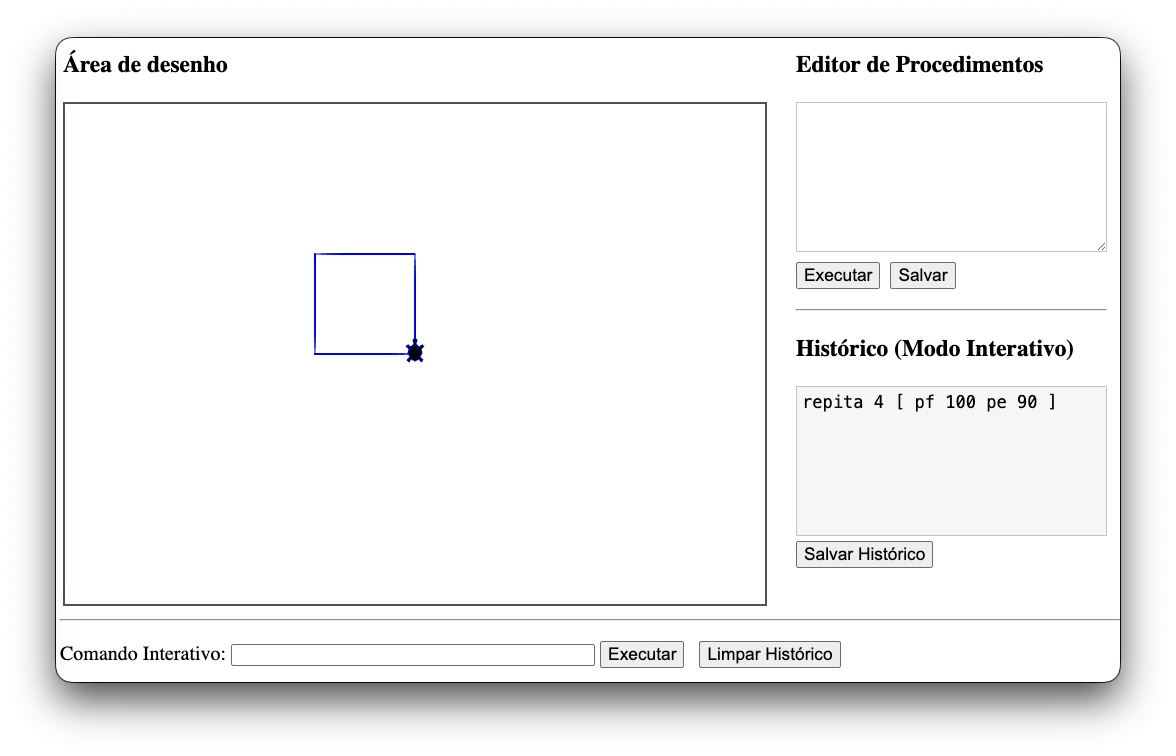
\includegraphics[width=1\textwidth]{imagem_exemplo_repita.png}
	    \label{fig:repita}
	 \end{figure}
	 
	 Veja um curto vídeo usando o comando \texttt{repita}: \href{https://youtu.be/TzylHqhVoho}{Comando \texttt{repita}.} 
	 
	 
	 \section{Comando Aprenda}
	 
	 O comando \textbf{\texttt{aprenda}} é utilizado para a criação de novos procedimentos, permitindo expandir o vocabulário de comandos reconhecidos pela tartaruga. A ideia é o que próprio comando transmite: ensinar a tartaruga novos comandos. O comando deve ser utilizado no Editor de Procedimentos. Vamos chamar o novo comando ensido de \textbf{procedimento}. 
	 
	 A estrutura é iniciada com a palavra-chave \textbf{\texttt{aprenda}}, seguida pelo nome do procedimento e, caso existam, pelos seus parâmetros identificados pelo caractere de dois-pontos (\texttt{:}). 
	 
	 Parâmetros são valores que o usuário digita quando chama o procedimento. Por exemplo, o comando \texttt{pf} exige um parâmetro, que é a quantidade de passos que a tartaruga deve andar para frente. Então na linha \texttt{pf 100}, temos o comando \texttt{pf} e o parâmetro \texttt{100}. Ao ``ensinar'' a tartaruga, podemos usar quantos parâmetros quisermos.
	 
	 Nas linhas a seguir colocamos os comandos que a tartaruga deve executar quando o procedimento for chamado no Editor de Procedimentos ou no Comando Interativo. O bloco de comandos é finalizado obrigatoriamente com a palavra \textbf{\texttt{fim}}.
	 
	 Uma dica: \textbf{tanto no nome do procedimento, quanto no nome dos parâmetros, exite usar símbolos (@, \#, \$, \%, etc.) e evite usar palavras com acento.}
	 
	 A sintaxe padrão é a seguinte:
	 \begin{verbatim}
	 	aprenda nome_do_procedimento :parametro1 :parametro2 ...
	 	comandos
	 	fim
	 \end{verbatim}
	 
	 O exemplo abaixo define o procedimento \texttt{quadrado}, que utiliza o comando \texttt{repita} para construir a figura geométrica com base em um parâmetro de tamanho, que chamamos de \texttt{:lado}:
	 
	 \begin{verbatim}
	 	aprenda quadrado :lado
	 	repita 4 [pf :lado pd 90]
	 	fim
	 \end{verbatim}
	 
	 Uma vez executado no Editor de Procedimentos, o novo comando passa a integrar a memória ativa da tartaruga, podendo ser chamado diretamente no Comando Interativo ou dentro de outros procedimentos apenas pelo nome estabelecido e acompanhado do valor do parâmetro, como no formato \texttt{quadrado 100}.
	 
	 Na Figura \ref{img:aprenda} criamos, no Editor de Procedimentos, o procedimento \texttt{quadrado}, que tem um único parâmetro: \texttt{:lado}. Em seguida usamos os seguintes comandos no Comando Interativo:
	 
	\begin{verbatim}
		quadrado 100
		un
		pt 200
		ul
		mudecl vermelho
		quadrado 50
	\end{verbatim}
	
	A tartaruga desenhou um quadrado de lado \texttt{100} (\texttt{quadrado 100}), em azul (cor original do \textsc{LogoAX}), levantou o lápis (\texttt{un}), andou \texttt{200} para tráz (\texttt{pt 200}), voltou a usar o lápis (\texttt{ul}), mudou a cor do lápis para \textcolor{red}{vermelho} e desenhou um quadrado de lado \texttt{50} (\texttt{quadrado 50}).
	 
	 
	\begin{figure}[H]
		\centering
		\caption{Exemplo de traçado geométrico utilizando a estrutura \texttt{aprenda}.}
		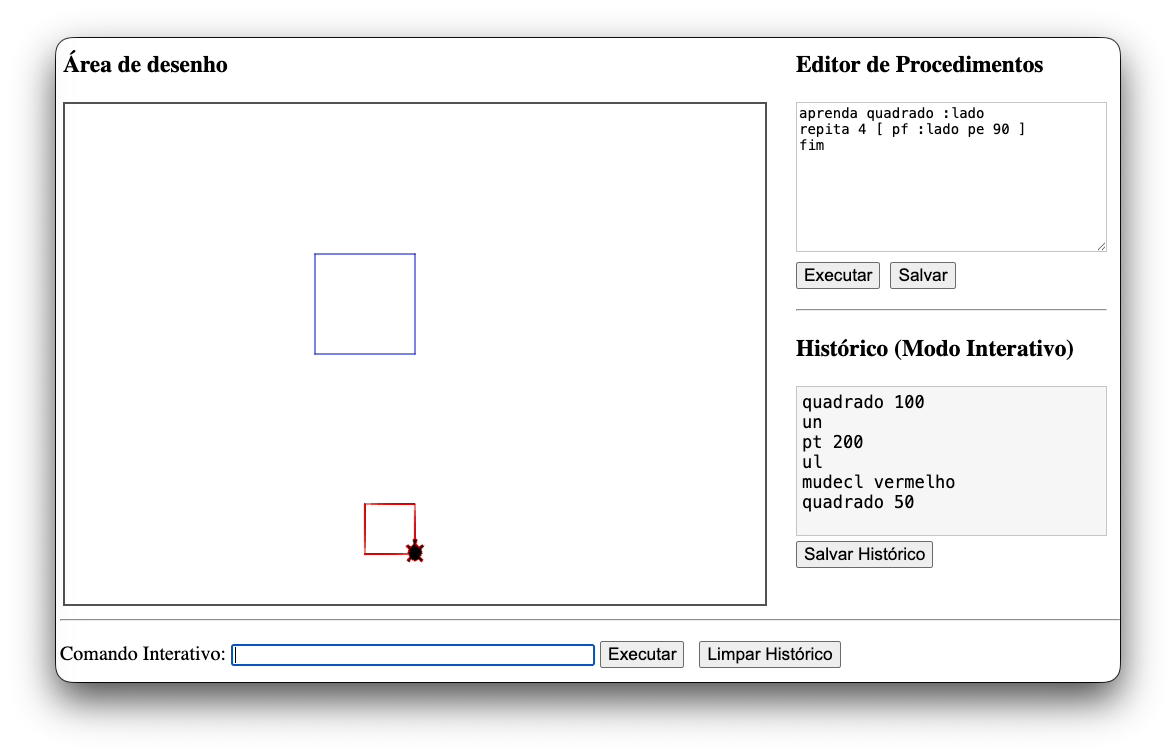
\includegraphics[width=1\textwidth]{imagem_exemplo_aprenda.png}
		\label{img:aprenda}
	 \end{figure}
	 
	 Fizemos também um vídeo com essa sequência de comandos: \href{https://youtu.be/J1RFn4tVK1I}{Comando \texttt{aprenda}}.

\end{document}